\documentclass[12pt,letterpaper]{article}
\usepackage[utf8]{inputenc}
\usepackage{amsmath}
\usepackage{amsfonts}
\usepackage{amssymb}
\usepackage{amsthm}
\usepackage{graphicx}
\usepackage{tabularx}
\usepackage[left=2cm,right=2cm,top=2cm,bottom=2cm]{geometry}
\usepackage{fancyhdr}
\usepackage{multicol}
\usepackage{multirow,array}
\usepackage{newtxtext,newtxmath}
\usepackage{relsize}
\usepackage{lastpage}
\usepackage{cancel}
\usepackage{tikz}
\usepackage{enumitem}
\usepackage{adjustbox}
\newcolumntype{Y}{>{\centering\arraybackslash}X}
\setenumerate[1]{label={\bf \theenumi: ~}}
\setenumerate[2]{label={\bf \theenumii: ~}}
\pagestyle{fancy}
\fancyhf{}
\lhead{\textsc{BHCC Mat-181}}
\rhead{\textsc{Binomial Distributions}}
\rfoot{Page \thepage ~of \pageref{LastPage}}

\newcommand*\circled[1]{\tikz[baseline=(char.base)]{
            \node[shape=circle,draw,inner sep=2pt] (char) {#1};}}
\newcommand{\N}[2]{\mathcal{N}\big(#1,~#2\big)}
\newcommand{\Geo}[1]{\texttt{Geo}\big(#1\big)}
\newcommand{\B}[2]{\mathcal{B}\big(#1,~#2\big)}

\begin{document} \large
\begin{enumerate}
\item Let $X\sim \B{48}{0.75}$. You want to estimate $P(33 \le X \le 40)$ using a normal approximation.
\begin{enumerate}
\item Calculate $\mu$.
\vfill
\item Calculate $\sigma$.
\vfill
\item Let $k$ represent possible values of $X$. Fill in the appropriate values of $k$ on the horizontal axis.

\vspace{20pt}
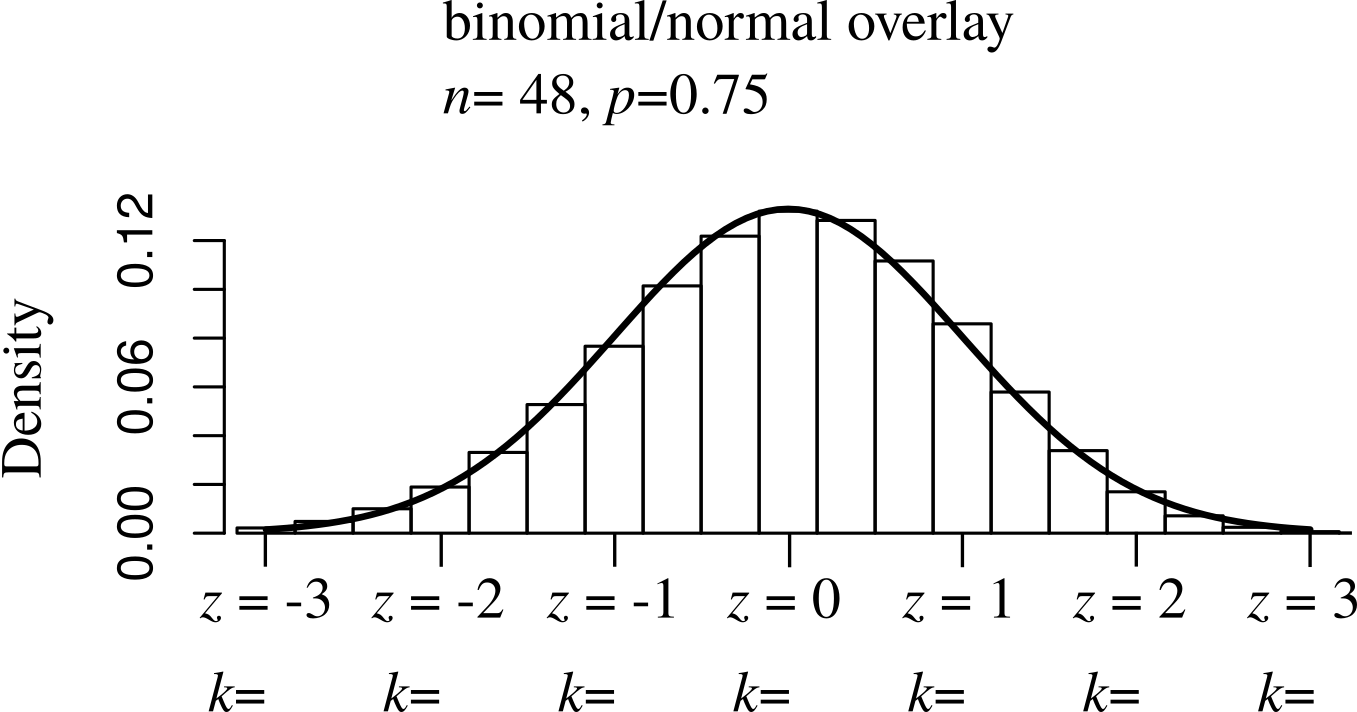
\includegraphics[scale=1.3]{nice_binos/prob1}
\vspace{5pt}
\item Shade the region denoted by $33 \le X \le 40$.
\vfill
\item Estimate $P(33 \le X \le 40)$ using the normal approximation. Be sure to make the \emph{continuity correction}.
\vfill
\end{enumerate}

\newpage

\item \begin{enumerate}
\item Let $X\sim \B{2500}{0.02}$. You want to estimate $P(40 < X < 48)$ using a normal approximation. Complete the diagram below (with horizontal axis values, associated $z$ scores, and a shaded area of $40 < X < 48$).

\hspace{-100pt}
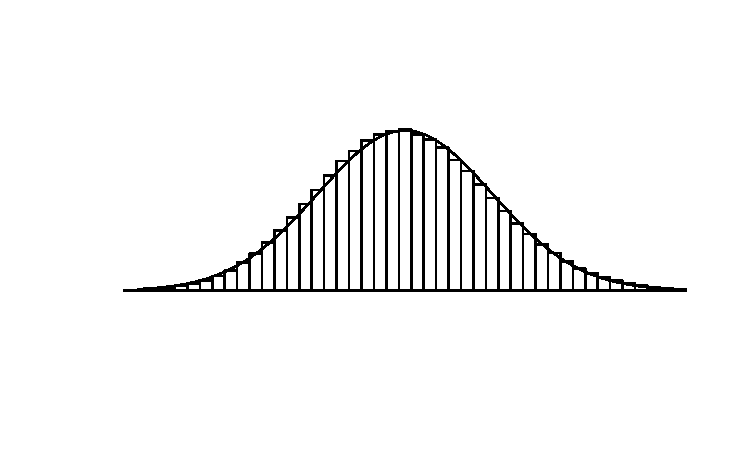
\includegraphics[scale=1.5]{nice_binos/overlay_2500_0p02.pdf}

\item Estimate $P(40 < X < 48)$ using the normal approximation. Be sure to make the \emph{continuity correction}.
\vfill
\item Based on the shaded figure, do you think the normal approximation is too high or too low?
\vfill
\end{enumerate}

\newpage

\item \begin{enumerate}
\item Let $X\sim \B{100}{0.8}$. You want to estimate $P(X \ge 85)$ using a normal approximation. Complete the diagram below (with horizontal axis values, associated $z$ scores, and a shaded area of $X \ge 85$).

\hspace{-100pt}
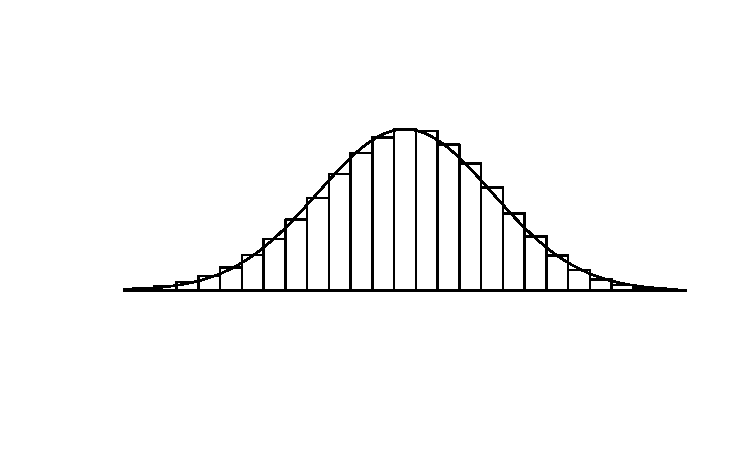
\includegraphics[scale=1.5]{nice_binos/overlay_100_0p8.pdf}

\item Estimate $P(X \ge 85)$ using the normal approximation. Be sure to make the \emph{continuity correction}.
\vfill
\end{enumerate}

\newpage

\item A fair coin is flipped 144 times.
\begin{enumerate}
\item What's the probability of getting exactly 72 heads?
\vfill
\item What's the probability that the first tails is the 4th flip?
\vfill
\item What's the probability of getting fewer than 72 heads? (You should be able to calculate this exactly, but a normal approximation will also be very good.)
\vfill
\item What's the probability that the number of heads is at least 60 and not more than 84?
\vfill
\end{enumerate}

\newpage

\item A coin will be spun 100 times. There is a question about whether the coin is fair. Before spinning the coin, we decide which outcomes will lead us to claim the coin unfair.

The null hypothesis is that the coin is fair, and any variation from 50 tails is just due to chance.  Under the null hypothesis, $X\sim\B{100}{0.5}$.
\begin{enumerate}
\item  According to the null hypothesis, what is the smallest integer $r$ such that $$P\Big(\big|X-50\big| > r\Big) ~~~~<~~~~ 0.05$$?
\vfill
\vfill
\item So...
\vfill

\end{enumerate}



\end{enumerate}
\end{document}

